\section{Optimization}
\label{sec:optimization}

\subsection{Mathematical formulation}
\label{sec:mathematical_formulation}
Optimization is the minimization or maximization of a function $f(x)$ subject to constraints $c_i(x) = 0, c_j(x) \ge 0$ on its variables $x \in \mathbb{R}^n$ \citep{nocedal2006numericaloptimization}. Minimization and maximization pose equivalent optimization problems, as minimizing $f(x)$ is the same as maximizing $-f(x)$. In this thesis, we will be solving minimization problems.

\subsection{Continuous and discrete optimization}
\label{sec:continuous_and_discrete_optimization}
In continuous optimization, the feasible set of solutions is uncountably infinite, such as the set of real numbers. These problems are usually easier to solve because of the smoothness of the optimization function, which makes it possible to deduce information about the function's behavior at all points close to a point $x$. On the other hand, in discrete optimization, the feasible set of solutions can be the set of integers, or of a more complex structure, such as permutations of an ordered set. These problems are typically harder to solve, because the behavior of the function can significantly change as we move from one feasible solution to another. In this thesis, we will be solving discrete optimization problems.

\subsection{Constrained and unconstrained optimization}
\label{sec:constrained_and_unconstrained_optimization}
If an optimization problem has at least one constraint $c_i(x) = 0$ or $c_i(x) \ge 0$, then the problem can be categorized as a constrained optimization problem. If the problem has no constraints, then it can be categorized as an unconstrained optimization problems. Constrained optimization problems are typically harder to solve, as the constraints can complicate the search process. In this thesis, we will be solving constrained problems.

\subsection{Global and local optimization}
\label{sec:global_and_local_optimization}
In local optimization problems, the goal is to find a solution that is better than all other feasible solutions which are close to the solution in the search space. On the other hand, in global optimization problems, the goal is to find the best solution among all feasible solutions. Global optimization problems are typically much harder to solve, especially if the optimization function is highly nonlinear, having many local optima. In this thesis, we will be solving global optimization problems.

\subsection{Deterministic and stochastic optimization}
\label{sec:deterministic_and_stochastic_optimization}
The algorithm used to search for a solution can be deterministic or stochastic. If it is deterministic, it will always yield the same results on a particular problem. On the other hand, if the algorithm is stochastic, it will use a random number generator when searching for a solution, and this means that different runs of the same algorithm will yield different results. In this thesis, we will be doing stochastic optimization.

\subsection{Example: The travelling salesman problem}
\label{sec:the_travelling_salesman_problem}
To demonstrate the types of problems we will solve in this thesis, we will go over the travelling salesman problem. The setup for this problem is that a salesman starts his journey in a city, has to visit every city exactly once, and has to return to the starting city. The goal is to minimize the distance that the traveller makes in his journey. In terms of graph theory, the goal is to find the shortest Hamiltonian cycle in the graph comprised of all the cities that the salesman has to visit. This problem is an NP-complete problem \citep{sipser2012computation}, meaning that no algorithm for solving it which runs in polynomial time is known.

The problem is discrete, as every permutation of the sets of cities represents one feasible solution. It is constrained, because the traveller can visit every city exactly once and return to the starting city at the end. The goal is to find the shortest Hamiltonian cycle, so this problem is global. Finally, the problem could be solved both deterministically and stochastically. A deterministic algorithm would go over all possible permutations of the set of cities to find the shortest cycle. While this algorithm would find the global optimum, the problem is intractable, meaning that after a certain point in the size of the problem, where size is measured in the number of cities that the traveller needs to visit, it would take unreasonably long time to terminate the algorithm. Instead, stochastic algorithms are used for solving larger problems.

In Figure \ref{fig:tsp}, a simple travelling salesman problem is demonstrated. The left image shows a grid of cities, and the right image shows the shortest Hamiltonian cycle in the grid. This figure, and all the subsequent figures in this thesis, were created using the draw.io software \citep{drawio}.

\begin{figure}[!htbp]
	\centering
	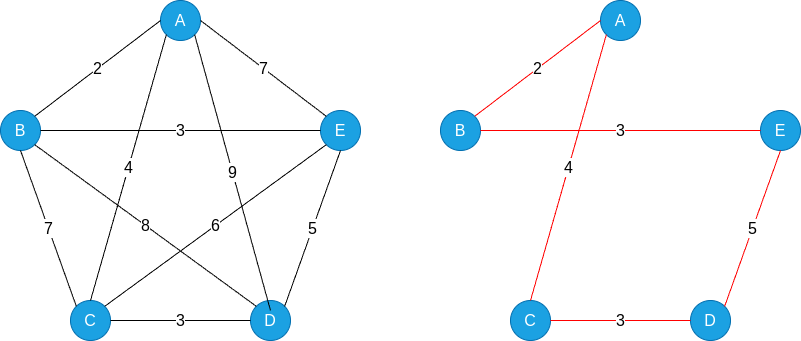
\includegraphics[scale=0.25]{../images/TSP.png}
	\caption{The travelling salesman problem}
    \label{fig:tsp}
\end{figure}